\documentclass{article} \usepackage{graphicx} \usepackage{hyperref}
\usepackage{listings} \usepackage{url}

\setlength{\parskip}{1em}

\begin{document}

\title{Building new ICE Item plugins}


\section{Setting up the new Item project} 

This tutorial will teach you how you
can create your own ICE Items via the built in tools within ICE.  The only
requirement for this tutorial is a sufficiently updated version of ICE.  

We will walk through the development of an item project for the FERN code.  To
begin, you will need to have a copy of FERN.  You can find installation
instructions for FERN at \url{https://github.com/jayjaybillings/fern}.

Then we will show you how you can incorporate these new plugins into your
installation of ICE and how to distribute them to others.  To begin launch ICE.
We will begin from a clean workbench.

\begin{center} 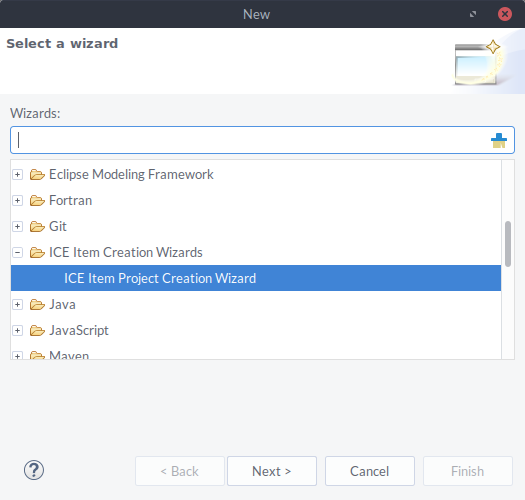
\includegraphics[width=8cm]{images/2} \end{center}

To create a new ICE Item project click the \texttt{New} button in the left hand
side of the toolbar.  From the wizard that appears you should find a section
called \texttt{ICE Item Creation Wizards}; open this and select \texttt{ICE
Item Creation Wizard} and click the \texttt{Next >} button.

\begin{center} 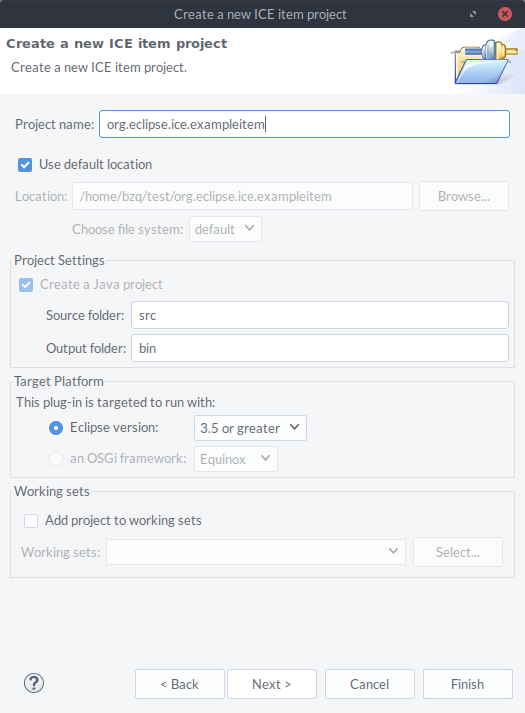
\includegraphics[width=8cm]{images/3} \end{center}

You will be met with a standard new project wizard page, in which you can name
your project.  We will call ours \texttt{org.eclipse.ice.fern}.  You do not
need to prefix your project with the \texttt{org.eclipse.ice} text, though we
do to showcase the packaging of the generated code.  Once you have named your
project click the \texttt{Next >} button.

\begin{center} 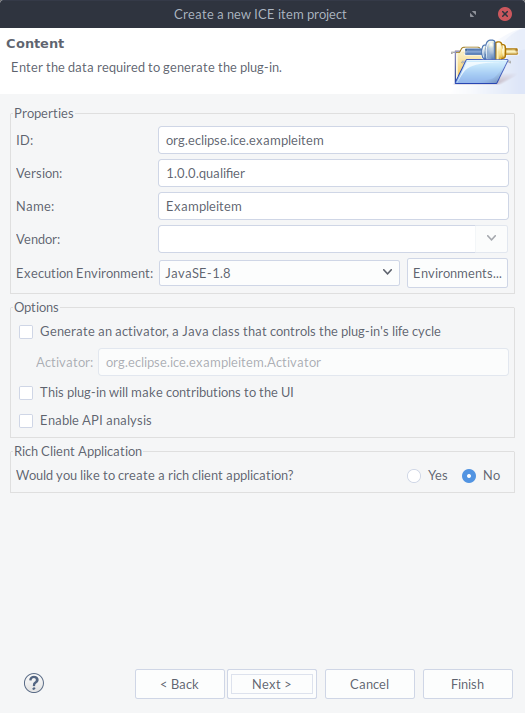
\includegraphics[width=8cm]{images/4} \end{center}

Now you are able to customize the plugin-specific portions of the project.  You
do not need to do anything at the point unless you have specific requirements.
We will simply go to the next page by clicking the \texttt{Next >} button
again.

\begin{center} 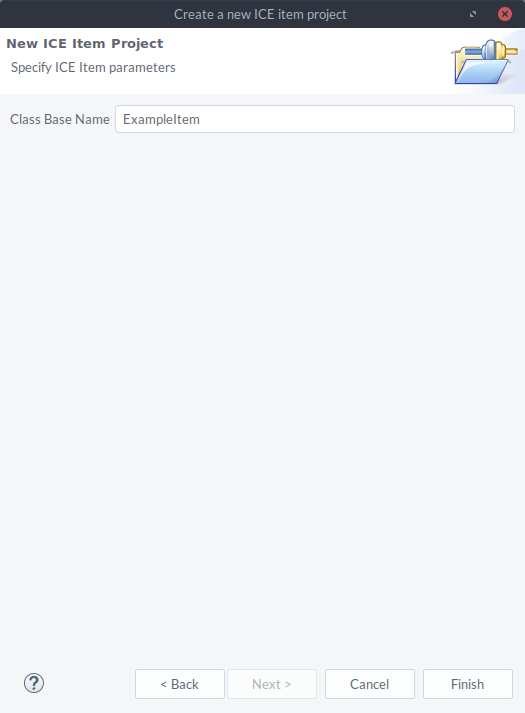
\includegraphics[width=8cm]{images/5} \end{center}

On this page you will have to tell the wizard what you want to use as a base
name for your item classes.  We will call it \texttt{Fern}, though you could
name it anything you want.  When you have entered your base class name you can
click the \texttt{Finish} button to generate your new item plugin project.

\begin{center} 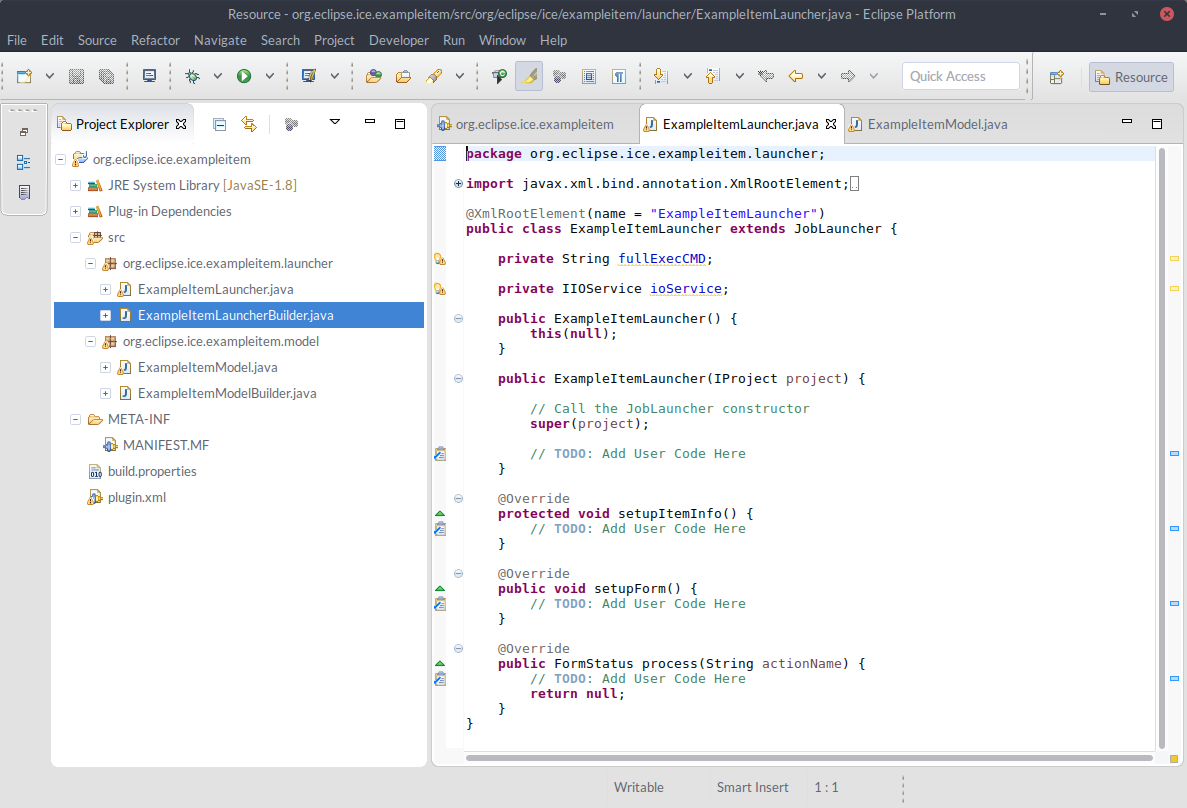
\includegraphics[width=12cm]{images/6} \end{center}

When the project has finished generating you should be able to explore the code
that has been created.  Within the source directory there will be two packages,
each containing two Java classes:

\begin{itemize} 
    \item \texttt{org.eclipse.ice.fern.launcher} 
    \begin{itemize}
        \item \texttt{FernLauncher.java} 
        \item \texttt{FernLauncherBuilder.java}
    \end{itemize} 
    \item \texttt{org.eclipse.ice.fern.model} 
    \begin{itemize} 
        \item \texttt{FernModel.java} 
        \item \texttt{FernModelBuilder.java}
    \end{itemize} 
\end{itemize}

To add functionality to the project you will only be responsible for editing
the \texttt{Launcher} and \texttt{Model} classes and can ignore the
\texttt{LauncherBuilder} and \texttt{ModelBuilder} classes.


\section{Adding functionality to the project}

\subsection{Completing the Model}

The Model (\texttt{FernModel.java}) will be responsible for creating and
validating input parameters for FERN.  In order to make the generated code run
there are several pieces of information that need to be changed.  First, we
will need to set up information that is necessary to process files for Fern.
The required variables are at the top of the \texttt{FernModel} class.  Change
them so that they say:

\begin{lstlisting}
private String writerName = "INIWriter";
private String readerName = "INIReader";
private String outputName = "fern_config.ini";
\end{lstlisting}

With the settings configured properly we can begin to implement the model set
up.  There are two pieces to this step.  First we will uncomment some code in
the \texttt{setupForm()} method:

\begin{lstlisting}
if (project != null)
    loadInput(null);
\end{lstlisting}

Uncommenting these lines will cause the \texttt{loadInput()} method to be
invoked on loading of the item no matter how it was created.  The \texttt{null}
argument simply means that we are not loading a predefined file.  To make this
work how we want, we will also have to modify the logic in the \texttt{loadInput()} 
method body:

\begin{lstlisting}[language=java]
if (readerName == "FernDefaultReaderName") {
    return;
}

// This is our new code
if (fileName == "null") {
    ContinuousEntry ce;
    StringEntry se;

    // Create the network section
    DataComponent networkComp = new DataComponent();
    networkComp.setName("Network");
    networkComp.setId(0);
    ce = new ContinuousEntry();
    ce.setName("numSpecies");
    ce.setValue("0");
    networkComp.addEntry(ce);
    ce = new ContinuousEntry();
    ce.setName("numReactions");
    ce.setValue("0");
    networkComp.addEntry(cd);
    ce = new ContinuousEntry();
    ce.setName("numReactionGroups");
    ce.setValue("0");
    networkComp.addEntry(ce); 
    ce = new ContinuousEntry();
    ce.setName("massTol");
    ce.setValue("0");
    se = new StringEntry();
    se.setName("networkFile");
    se.setValue("/home/user/input.inp");
    networkComp.addEntry(se);
    se = new StringEntry();
    se.setName("rateFile");
    se.setValue("/home/user/data.data");
    networkComp.add(se);
    
    // Create the initial conditions section
    DataComponent initConditionsComp = new DataComponent();
    initConditionsComp.setName("Initial Conditions");
    initConditionsComp.setId(1);
    ce = new ContinuousEntry();
    ce.setName("T9");
    ce.setValue("0");
    initConditionsComp.addEntry(ce);
    ce = new ContinuousEntry();
    ce.setName("startTime");
    ce.setValue("0");
    initConditionsComp.addEntry(ce);
    ce = new ContinuousEntry();
    ce.setName("endTime");
    ce.setValue("0");
    initConditionsComp.addEntry(ce);
    ce = new ContinuousEntry();
    ce.setName("initialTimeStep");
    ce.setValue("0");
    initConditionsComp.addEntry(ce);
    ce = new ContinuousEntry();
    ce.setName("density");
    ce.setValue("0");
    initConditionsComp.addEntry(ce);
    form.add(initConditionsComp);
} else {
    IFile inputFile = project.getFile(fileName);
    reader = ioService.getReader(readerName);
    form = reader.read(inputFile);
}
form.setName(getname());
form.setDescription(getDescription());
form.setId(getId());
form.setItemID(getId());
\end{lstlisting}


\subsection{Completing the Launcher}
The launcher handles the actual running of the FERN code.  In order to make it work we will have to provide information about how to run FERN.  In this case we can simply edit the \texttt{execCommand} variable:

\begin{lstlisting}[language=java]
execCommand = ${installDir}fern-exec ${inputFile}
\end{lstlisting}

\section{Building and incorporating your item into ICE}
Todo

\end{document}

